\documentclass[10pt,a4paper]{article}

% ---- 页面布局 ----
\usepackage[includehead=true,includefoot=true,centering]{geometry}
\geometry{left=2.5cm,right=2.5cm,top=2.5cm,bottom=2.5cm}

% ---- 中文支持 ----
\usepackage[heading=true,fontset=none]{ctex}

% ---- 字体 ----
\usepackage{fontspec}
\setmainfont{Times New Roman}
\IfFontExistsTF{Source Han Serif CN}
  {\setCJKmainfont{Source Han Serif CN}}
  {\IfFontExistsTF{Noto Serif CJK SC}
    {\setCJKmainfont{Noto Serif CJK SC}}
    {\IfFontExistsTF{SimSun}
      {\setCJKmainfont{SimSun}}
      {\setCJKmainfont{FangSong}}}}

% ---- 数学与化学 ----
\usepackage{amsmath,amssymb}
\usepackage{amsfonts}
\usepackage[version=4]{mhchem}
\usepackage{stmaryrd}
\usepackage{bbold}

% ---- 颜色与超链接 ----
\usepackage{xcolor}
\usepackage{hyperref}
\hypersetup{
  colorlinks=true,
  linkcolor=blue,
  filecolor=magenta,
  urlcolor=cyan
}
\urlstyle{same}

% ---- 图表 ----
\usepackage{graphicx}
\usepackage[export]{adjustbox}
\usepackage{booktabs}
\usepackage{longtable}
\usepackage{array}
\usepackage{tabularx}
\usepackage{colortbl}
\definecolor{table-rule-color}{HTML}{999999}
\arrayrulecolor{table-rule-color}

% ---- 列表 ----
\usepackage{enumitem}
\setlist{nosep,leftmargin=*}

% ---- 行距与段落 ----
\usepackage{setspace}
\setstretch{1.3}
\setlength{\parindent}{2em}
\setlength{\parskip}{4pt plus 2pt minus 1pt}

% ---- 页眉页脚 ----
\usepackage{fancyhdr}
\pagestyle{fancy}
\fancyhf{}
\fancyhead[C]{RAG-Lab 检索增强生成实验报告}
\fancyfoot[C]{\thepage}
\renewcommand{\headrulewidth}{0.4pt}

% ---- 脚注 ----
\usepackage{footnote}
\makesavenoteenv{longtable}

% ---- 其他工具 ----
\usepackage{calc}
\usepackage{etoolbox}
\setlength{\emergencystretch}{3em}

% ---- Pandoc 兼容宏 ----
\makeatletter
\newsavebox\pandoc@box
\newcommand*\pandocbounded[1]{%
  \sbox\pandoc@box{#1}%
  \Gscale@div\@tempa{\textheight}{\dimexpr\ht\pandoc@box+\dp\pandoc@box\relax}%
  \Gscale@div\@tempb{\linewidth}{\wd\pandoc@box}%
  \ifdim\@tempb\p@<\@tempa\p@\let\@tempa\@tempb\fi%
  \ifdim\@tempa\p@<\p@\scalebox{\@tempa}{\usebox\pandoc@box}%
  \else\usebox{\pandoc@box}%
  \fi%
}
\def\fps@figure{htbp}
\makeatother

\providecommand{\tightlist}{%
  \setlength{\itemsep}{0pt}\setlength{\parskip}{0pt}}

\author{}
\date{}

\begin{document}

% ============================================================
% 封面
% ============================================================
\begin{titlepage}
\thispagestyle{empty}
\begin{center}

% 1. 校徽
\includegraphics[width=3cm]{whu-logo.png}

\vspace{0.5cm}

% 2. 学校名称
{\Huge\bfseries 武汉大学}

\vspace{1.5cm}

% 3. 报告主标题
{\Huge\bfseries RAG-Lab 检索增强生成}

\vspace{1cm}

% 4. 课程信息
{\Large Python语言程序设计}

\vspace{0.3cm}
{\Large 课程项目报告}

\vspace{5cm}

% 5. 个人信息
\begin{tabular}{cc}
\large 专业名称 & \large 数据科学与大数据技术 \\
\large 课程名称 & \large Python语言程序设计 \\
\large 指导教师 & \large 刘纪平 \\
\large 学生学号 & \large 2024302011056 \\
\large 学生姓名 & \large 唐佳霂 \\
\end{tabular}

\vspace{2.5cm}

% 6. 日期
{\large 2026年5月11日}

\vspace{0.5cm}
\textbf{项目开源地址：} \url{https://github.com/jmdonbaba/RAG-Lab}

\end{center}
\end{titlepage}


% ---- 此后恢复页眉 ----
\thispagestyle{fancy}

% ============================================================
% 摘要
% ============================================================
\section*{摘\quad 要}
\addcontentsline{toc}{section}{摘要}

本实验围绕基于Python的检索增强生成（Retrieval-Augmented Generation, RAG）系统的设计与实现展开。RAG-Lab项目从底层实现了从文档抓取、文本分块、向量嵌入、向量数据库构建到混合检索与LLM答案生成的完整RAG流水线。系统以CMU 10-701机器学习课程公开讲义为知识库，支持三种文本分块策略（固定Token分块、递归字符分块、语义分块），集成ChromaDB和FAISS两种向量存储后端，实现BM25关键词检索与向量语义检索的混合检索方案（RRF融合），并通过DeepSeek/OpenAI API实现基于检索文档的答案生成。系统提供CLI命令行和Gradio网页两种交互方式，内置完整的评估功能，支持检索质量、分块策略、嵌入模型的多维度对比分析。通过本实验，深入掌握了RAG系统的核心原理与实现技术，包括文档处理流程、向量嵌入模型应用、向量数据库操作、混合检索策略、LLM API调用与提示词工程等，具备了一个完整可用的检索增强生成系统的构建能力。

\medskip
\noindent\textbf{关键词：}检索增强生成（RAG）；向量数据库；混合检索；大语言模型；ChromaDB；Sentence-Transformers；Gradio

\newpage

% ============================================================
% 目录
% ============================================================
\section*{目\quad 录}
\addcontentsline{toc}{section}{目录}
\renewcommand{\contentsname}{}
\tableofcontents

\newpage

% ============================================================
% 第1章 引言
% ============================================================
\section{引言}

\subsection{选题背景}

大语言模型（Large Language Model, LLM）近年来取得了突破性进展，以DeepSeek、GPT系列为代表的模型展现出强大的自然语言理解与生成能力。然而LLM存在两个根本性缺陷：一是知识截止日期限制——模型训练数据具有时效性，无法回答训练截止日期之后出现的新问题；二是幻觉（Hallucination）问题——模型在缺乏可靠信息来源时可能编造不存在的事实，表面合理但实际错误。

检索增强生成（Retrieval-Augmented Generation, RAG）应运而生，其核心思路是"先检索，再生成"：当用户提出问题时，系统首先从外部知识库中检索相关文档片段，然后将检索到的内容作为上下文提供给LLM，使模型能够基于真实资料生成答案。这种方法有效解决了LLM的知识时效限制和幻觉问题，已成为生产环境中大模型应用的标准架构之一。

当前，RAG技术在工业知识问答、智能客服、学术研究辅助等领域得到了广泛应用。然而，RAG系统的构建涉及文档处理、文本分块、向量嵌入、相似度检索、混合检索融合、提示词工程等多个技术环节，学习门槛较高。因此，构建一个模块化、可交互的RAG实验系统，帮助学习者从原理到实践掌握RAG技术，具有重要的教学价值。

\subsection{选题内容}

本实验选题为"RAG-Lab：检索增强生成动手实验系统"，是一套基于Python语言开发的面向RAG学习与实验的平台。系统以卡内基梅隆大学（CMU）10-701机器学习课程（Spring 2011）的43篇公开PDF讲义为知识库，实现了从文档抓取、文本预处理与分块策略、向量嵌入、向量数据库构建、混合检索到LLM答案生成的完整RAG流水线。

系统的核心功能包括：（1）自动从CMU课程网站抓取并下载讲义PDF，解析提取纯文本；（2）实现三种文本分块策略——固定Token分块、递归字符分块和语义分块，支持策略对比分析；（3）集成Sentence-Transformers嵌入模型（BGE、M3E、MiniLM），将文本块转化为向量表示；（4）支持ChromaDB（持久化）和FAISS（纯内存）两种向量存储后端；（5）实现BM25关键词检索与向量语义检索的混合检索方案，通过RRF（Reciprocal Rank Fusion）算法融合排序；（6）通过DeepSeek/OpenAI API实现基于检索文档的LLM答案生成，包含提示词模板和来源追溯功能；（7）提供CLI命令行和Gradio网页两种交互界面；（8）内置完整评估功能，支持检索质量、分块策略、嵌入模型的多维度对比。

\subsection{选题价值}

本课题的研究与开发具有以下多方面的重要价值与实际应用意义：

\textbf{（1）提供系统化的RAG学习路径。}项目将RAG技术分解为文档加载、分块、嵌入、索引、检索、生成六个阶段，每个阶段对应独立的Python模块和Jupyter教程Notebook，使学习者能够循序渐进地掌握RAG各环节的技术细节。

\textbf{（2）展示工业级RAG系统的关键技术。}系统实现了混合检索（BM25 + 向量）、RRF融合、查询翻译、多策略分块等生产环境中常用的技术方案，具有较高的工程参考价值。

\textbf{（3）支持多维度的实验对比分析。}通过内置的评估功能，学习者可以量化对比不同分块策略、嵌入模型、检索方式的性能差异，培养数据驱动的系统优化思维。

\textbf{（4）良好的实用性与扩展性。}CLI工具方便开发验证与自动化脚本，Gradio网页界面支持直观交互与演示。模块化架构便于学习者根据需求替换或扩展组件（文档源、嵌入模型、LLM后端等）。

\textbf{（5）契合"学以致用"的Python教学导向。}项目综合运用了Python网络爬虫（requests, BeautifulSoup）、文档处理（pypdf）、数值计算（numpy）、API调用（openai SDK）、Web应用（gradio）等核心库，是Python程序设计课程的理想综合实践选题。

% ============================================================
% 第2章 系统需求分析
% ============================================================
\section{系统需求分析}

\subsection{概述}

\subsubsection{编写目标}

本文档旨在明确RAG-Lab系统的功能需求、质量要求与技术指标，为系统的设计、开发、测试和维护提供规范指导。通过需求文档，开发人员能够清楚理解系统的建设目标与功能范围，确保系统在后续的各项工作中保持一致性、可追溯性与可验证性。

\subsubsection{项目背景}

随着大语言模型的广泛应用，检索增强生成（RAG）技术已成为提升模型回答准确性和可信度的核心手段。然而，RAG涉及多个技术组件协同工作，缺乏系统化的学习工具。现有的RAG框架（如LangChain、LlamaIndex）功能全面但封装过度，不利于理解底层原理。为此，本项目采用Python语言，从底层实现RAG全过程，构建一个透明、可交互的学习实验系统，帮助学习者深入掌握RAG的核心技术原理与实现方法。

\subsubsection{术语与定义}

\begin{enumerate}[label=(\arabic*)]
\item RAG（Retrieval-Augmented Generation）：检索增强生成，一种结合信息检索与文本生成的AI技术架构。
\item 向量嵌入（Embedding）：将文本映射到高维向量空间的表示方法，语义相近的文本对应相似的向量。
\item 文本分块（Chunking）：将长文档切分为适合嵌入模型处理的短文本片段的过程。
\item BM25：一种基于词频统计的关键词检索算法，是TF-IDF的改进版本。
\item RRF（Reciprocal Rank Fusion）：基于排名融合的多路检索结果合并算法。
\item ChromaDB：开源嵌入式向量数据库，支持持久化存储与向量相似度检索。
\item FAISS：Meta开源的高性能向量相似度搜索库。
\item Sentence-Transformers：基于Transformer架构的句子嵌入模型库。
\item Gradio：用于构建机器学习模型演示界面的Python库。
\item LLM（Large Language Model）：大语言模型，如DeepSeek、GPT系列。
\end{enumerate}

\subsection{功能需求}

\subsubsection{系统功能概述}

本系统为一个基于Python语言开发的检索增强生成（RAG）学习实验平台，通过模块化设计，帮助学习者从原理到实践掌握RAG技术的各个环节。系统整体功能结构包含以下核心功能模块：

\textbf{（1）文档获取与解析模块}
\begin{itemize}
\item 支持从CMU 10-701课程网页自动抓取讲义链接列表
\item 支持PDF文件的批量下载与本地缓存管理
\item 支持PDF文件文本提取（使用pypdf实现）
\item 支持HTML文件解析与文本清洗
\item 解析结果以JSON格式持久化存储，避免重复处理
\item 离线环境下自动使用内置的10篇示例机器学习文档
\end{itemize}

\textbf{（2）文本分块模块}
\begin{itemize}
\item 支持三种分块策略：固定Token分块（基于tiktoken计数）、递归字符分块（按段落/句子/词/字符优先级递归切分）、语义分块（按句子边界切分，保持语义完整性）
\item 可配置分块大小（chunk\_size，默认512字符）和重叠量（chunk\_overlap，默认50字符）
\item 分块结果包含元数据（源文档、编号、策略类型等），支持溯源
\end{itemize}

\textbf{（3）向量嵌入模块}
\begin{itemize}
\item 支持多种Sentence-Transformers嵌入模型：all-MiniLM-L6-v2（英文轻量，384维）、BAAI/bge-small-zh-v1.5（BGE中文，512维）、moka-ai/m3e-base（M3E中文，768维）
\item 嵌入结果自动L2归一化，确保余弦相似度计算准确性
\item 支持批量嵌入与单条查询嵌入两种模式
\end{itemize}

\textbf{（4）向量存储与索引模块}
\begin{itemize}
\item 支持ChromaDB持久化存储（基于SQLite，适合反复使用）和FAISS内存存储（高性能，适合快速实验）两种后端
\item ChromaDB支持集合管理、数据清除与重建
\item FAISS使用内积索引（Inner Product），结合归一化向量实现余弦相似度计算
\end{itemize}

\textbf{（5）混合检索模块}
\begin{itemize}
\item 同时执行BM25关键词检索和向量语义检索，取两者之长
\item 支持RRF（Reciprocal Rank Fusion）排名融合和加权求和两种融合策略
\item 中文查询自动翻译为英文（通过DeepSeek API），解决跨语言BM25检索问题
\item 支持检索方式对比：单独BM25、单独向量、混合检索三种模式结果并排展示
\end{itemize}

\textbf{（6）LLM生成模块}
\begin{itemize}
\item 基于检索到的文档内容生成答案，使用结构化提示词模板（角色设定 + 上下文 + 问题 + 格式要求）
\item 支持DeepSeek API和OpenAI API两种LLM后端（通过统一OpenAI SDK接口调用）
\item 支持仅检索模式（\texttt{--no\_llm}），不调用LLM，直接展示检索到的文档片段
\item API调用失败时自动降级为模板化回复
\end{itemize}

\textbf{（7）系统评估模块}
\begin{itemize}
\item 检索质量评估：检索延迟、BM25与向量检索一致性（Jaccard系数）、融合得分分布
\item 分块策略对比：在不同文档集上对比三种分块策略的块数量、平均长度、检索延迟、BM25-向量一致性，评估前后自动恢复原始索引状态
\item 嵌入模型对比：比较不同嵌入模型的维度、平均相似度、区分度比率（最佳匹配/平均，可跨模型比较）
\item 生成质量评估：通过LLM实际生成回答，测量平均回答长度、平均使用来源数
\end{itemize}

\textbf{（8）用户界面模块}
\begin{itemize}
\item CLI命令行界面：提供build（构建索引）、query（单次问答）、compare（检索对比）、evaluate（运行评估）、ui（启动网页界面）五个子命令
\item Gradio网页界面：提供智能问答（ChatInterface）、检索对比（三列结果展示）、系统评估（一键运行）、关于系统四个功能页签
\item 网页界面采用现代设计语言，自定义CSS样式，支持响应式布局
\end{itemize}

\subsubsection{系统运行时序关系说明}

为直观说明系统各模块之间的调用关系与执行顺序，本系统定义如下RAG查询时序流程：

\begin{enumerate}[label=(\arabic*)]
\item 用户通过CLI或Web界面输入查询问题
\item Retriever模块接收查询，并行执行BM25检索（含中文预翻译）和向量检索（查询嵌入 $\to$ 向量相似度搜索）
\item 两路检索结果通过RRF或加权融合算法合并排序，返回Top-K文档片段
\item Generator模块将检索到的文档与用户问题组合，填入提示词模板
\item 提示词通过API发送至LLM（DeepSeek/OpenAI），生成基于文档的答案
\item 系统将答案、引用来源、检索耗时等信息一并返回给用户并展示
\end{enumerate}

\subsubsection{用户角色与用例}

RAG-Lab系统的用户主要为学习者和开发者，主要包括以下用例：
\begin{itemize}
\item 知识库构建：用户执行build命令（首次使用或Web界面启动时），系统自动完成文档抓取、分块、嵌入、索引构建全过程
\item 知识问答：用户提出机器学习相关问题，系统检索相关讲义内容并生成基于文档的回答
\item 检索策略对比：用户输入查询，系统并行展示BM25、向量、混合三种检索方式的Top-5结果
\item 系统评估：用户运行评估流程，系统自动执行多维度评测并生成对比报告
\end{itemize}

\subsubsection{核心数据对象}

RAG-Lab系统的核心数据实体包括：
\begin{itemize}
\item 文档（Document）：知识库的基本单元。包含源文件名称、文件路径、原始文本内容、文本长度等属性。系统以CMU课程讲义为文档源，每篇PDF讲义对应一个文档实体。
\item 文本块（Chunk）：检索的基本单元。由文档按策略切分后的片段，包含唯一ID（格式：文档名\_chunk\_编号）、所属文档名、文本内容、长度、分块策略等属性。每个文档被切分为多个文本块。
\item 向量嵌入（Embedding）：文本块的数值向量表示。每个文本块对应一个向量（384/512/768维）。存储于ChromaDB或FAISS索引中，用于相似度计算。
\item 检索结果（Retrieval Result）：检索返回的文本块，包含ID、内容、源文档、相关度得分、检索来源（BM25/向量/混合）等信息。
\end{itemize}

\subsection{非功能需求}

\subsubsection{性能需求}
\begin{itemize}
\item 系统应具备良好的响应速度与处理能力：在包含10-50篇文档的知识库上，单次检索延迟不超过500ms，端到端问答（含LLM调用）延迟不超过10秒
\item 批量嵌入处理支持小批量模式（默认batch\_size=32），在普通CPU环境下，43篇PDF文档的首次构建总耗时不超过5分钟
\item Gradio网页界面需保持流畅性，页面加载和交互响应无明显卡顿
\end{itemize}

\subsubsection{功能完整性需求}
\begin{itemize}
\item 系统功能模块覆盖完整且结构清晰，需覆盖文档获取、文本分块、向量嵌入、向量库构建、混合检索、答案生成、系统评估全流程
\item 提供CLI和Web两种等价交互方式
\item 离线环境下可借助内置示例数据运行核心功能
\end{itemize}

\subsubsection{安全需求}
\begin{itemize}
\item API Key安全：LLM API密钥通过.env环境变量文件配置，不硬编码在源代码中；.env文件已加入.gitignore防止泄露
\item 数据安全：文档和索引数据均存储在本地data/目录，已gitignore，不会被提交
\item 输入安全：CLI和Web输入均经过参数校验，防止注入攻击
\end{itemize}

\subsubsection{可维护性需求}
\begin{itemize}
\item 系统采用模块化设计，每个RAG环节对应独立的Python模块（document\_loader.py、chunker.py、embedder.py、vector\_store.py、retriever.py、generator.py、evaluator.py、app.py），功能边界清晰
\item 全部配置集中在config.py中，所有可调参数通过dataclass管理，附带详细注释，易于修改
\item 代码遵循Python编码规范，函数签名和类结构清晰，便于维护
\end{itemize}

\subsubsection{可扩展性需求}
\begin{itemize}
\item 分块策略采用策略模式（ChunkingStrategy抽象基类），新增策略只需继承基类并实现split方法
\item 向量存储采用统一接口（VectorStore类），新增存储后端（如Milvus、Pinecone）只需扩展存储初始化与查询方法
\item LLM后端支持通过provider参数切换（deepseek/openai/local），新增提供商只需扩展Generator类
\item 知识库文档源可通过修改config.py中的cmu\_lectures\_url配置接入其他网页文档
\end{itemize}

\subsubsection{易用性需求}
\begin{itemize}
\item 命令行界面提供完整的帮助信息（--help）和使用示例（epilog），支持参数合法性校验
\item Gradio网页界面采用现代设计语言，包含智能问答、检索对比、系统评估、关于系统四个功能页签
\item 网页色彩采用现代风格（蓝色主色调+灰色搭配），卡片式布局，圆角设计，交互元素状态明确
\item 检索来源以卡片形式展示，标注源文档名和相关度标签，提供内容预览，便于用户追溯信息来源
\end{itemize}

\subsection{技术选型}

本系统根据功能需求与工程应用场景，选择以下关键技术：

\subsubsection{编程语言}
使用Python 3.10+作为核心开发语言，充分利用Python在数据处理、机器学习、Web开发等领域的丰富生态。

\subsubsection{文档处理}
使用pypdf解析PDF文档，BeautifulSoup解析HTML网页与文本清洗，requests处理HTTP请求与文件下载。

\subsubsection{文本分块}
使用tiktoken库（OpenAI开源）进行Token级精确分块，并实现递归字符分块与语义分块策略。

\subsubsection{嵌入模型}
使用sentence-transformers库加载预训练嵌入模型，支持BGE系列（BAAI/bge-small-zh-v1.5）、M3E系列（moka-ai/m3e-base）、MiniLM系列（all-MiniLM-L6-v2）等模型。

\subsubsection{向量存储}
使用ChromaDB（嵌入式向量数据库，基于SQLite持久化，适合反复使用）和FAISS（Meta高性能向量搜索库，纯内存计算，适合快速实验）。

\subsubsection{关键词检索}
使用rank-bm25实现BM25关键词检索，jieba处理中文分词，DeepSeek API进行中→英跨语言查询翻译。

\subsubsection{LLM调用}
使用openai Python SDK统一调用DeepSeek API和OpenAI API（两者均兼容OpenAI接口格式），temperature参数设为0.1以降低幻觉。

\subsubsection{用户界面}
使用Gradio 4.x构建Web交互界面，argparse构建CLI命令行界面。Gradio提供ChatInterface、Dataframe、JSON等高级组件。

\subsubsection{评估与数据处理}
使用numpy进行数值计算与统计分析，scikit-learn提供评估指标计算。

\subsection{质量要求}

\subsubsection{可靠性与稳定性}
\begin{itemize}
\item 系统应具备较高的可靠性：文档下载失败或API调用异常时提供合理的错误提示和降级策略（内置示例文档、fallback模板回复）
\item 批量文档处理应具备容错能力，单篇文档处理失败不影响整体流程
\item ChromaDB持久化索引支持清除与重建，避免数据累积
\end{itemize}

\subsubsection{交付要求}
\begin{itemize}
\item 交付物为Python源代码，包含8个功能模块（document\_loader、chunker、embedder、vector\_store、retriever、generator、evaluator、app）、CLI入口（main.py）、全局配置（config.py）
\item 提供requirements.txt依赖清单、.env.example配置模板
\item 提供README.md项目说明文档、Jupyter Notebook教程、本实验报告
\item 代码结构清晰，模块划分合理，具备良好的可维护性与可扩展性
\end{itemize}

% ============================================================
% 第3章 系统设计
% ============================================================
\section{系统设计}

\subsection{概述}

\subsubsection{项目背景}

随着大语言模型的快速发展，让模型获取最新、准确的外部知识成为AI应用的关键挑战。RAG技术通过将信息检索与文本生成相结合，为这一挑战提供了有效的解决方案。然而，RAG系统的构建涉及多个技术组件协同工作，学习者的上手机门槛较高。因此，设计一套从底层实现的RAG实验系统，帮助学习者理解每个环节的原理与实现细节，具有重要的教学与实践价值。

\subsubsection{项目目标与意义}

本项目旨在设计并实现一个模块化、可交互的RAG学习实验系统。通过将RAG流水线拆解为循序渐进的六个阶段，每个阶段对应独立的Python模块，使学习者能够逐步掌握RAG各项核心技术原理，对比不同分块策略、嵌入模型和检索方式的效果差异，理解向量数据库、混合检索等核心技术的实现方法，获得构建实际RAG应用的工程能力。

\subsubsection{项目预期目标}

\begin{enumerate}[label=(\arabic*)]
\item 实现从文档抓取到答案生成的完整RAG流水线
\item 支持多种分块策略、嵌入模型和向量存储后端的灵活切换与对比
\item 实现BM25+向量的混合检索（RRF融合），达到比单一检索更好的效果
\item 提供CLI和Gradio Web两种交互界面，兼顾开发效率与演示效果
\item 内置完整评估功能，支持检索质量、分块策略、嵌入模型的多维度量化对比
\item 系统架构模块化、参数可配置，便于替换和扩展
\end{enumerate}

\subsubsection{设计原则与方法}

\begin{enumerate}[label=(\arabic*)]
\item 模块化设计：系统按RAG流水线阶段划分为独立模块，模块间通过明确接口交互，降低耦合度
\item 策略模式：分块策略采用抽象基类+多态实现，支持运行时切换策略
\item 配置集中化：所有参数集中在config.py的Config dataclass中管理，通过环境变量注入敏感信息
\item 统一接口：向量存储（ChromaDB/FAISS）、LLM后端（DeepSeek/OpenAI）均通过统一的外部接口调用，屏蔽底层差异
\item 容错设计：关键外部依赖（文档下载、API调用）均有降级策略，确保核心功能在异常情况下仍可运行
\end{enumerate}

\subsection{系统功能设计}

\subsubsection{系统结构总览}

本系统采用分层架构设计，基于Python语言，结合多种开源库实现RAG全过程：

\begin{enumerate}[label=(\arabic*)]
\item 表示层（UI层）：通过Gradio实现Web交互界面（ChatInterface + Tabs布局），通过argparse实现CLI命令行界面，负责用户输入收集与结果展示
\item 业务逻辑层：系统核心功能层，包含文档加载、文本分块、向量嵌入、混合检索、LLM生成和系统评估六个模块，各模块通过Pipeline类协调调度
\item 数据持久层：包括向量数据库与文件系统。ChromaDB基于SQLite实现向量存储，JSON文件存储已解析的文档文本，文件系统存储原始PDF/HTML文件
\end{enumerate}

\subsubsection{系统模块划分与功能简介}

系统整体功能采用模块化设计，分为以下核心模块，各模块相互独立，通过RAGPipeline统一调度：

\textbf{（1）文档加载模块（DocumentLoader）}

负责从CMU课程网页抓取链接、批量下载PDF文件、提取纯文本并清洗存储。支持PDF（pypdf）和HTML（BeautifulSoup）两种格式解析。解析结果以JSON格式保存，避免重复处理。内置10篇示例机器学习文档确保离线可用。

\textbf{（2）文本分块模块（Chunker）}

提供三种分块策略：FixedTokenChunker基于tiktoken编码实现Token级精确分块；RecursiveCharChunker按段、句、词、字符优先级递归切分，优先保持段落和句子完整性；SemanticChunker按句子边界切分并聚合至目标长度，保持语义完整性。所有策略支持chunk\_size和chunk\_overlap灵活配置。

\textbf{（3）向量嵌入模块（Embedder）}

基于sentence-transformers库，封装多种嵌入模型的加载与调用。支持批量嵌入（encode方法）和单条查询嵌入（embed\_query方法），嵌入结果自动L2归一化。提供compare\_embedding\_models工具函数，用于对比不同模型在相同文本集上的相似度分布与区分度比率（最佳匹配/平均相似度，可跨模型比较）。

\textbf{（4）向量存储模块（VectorStore）}

统一封装ChromaDB和FAISS两种向量存储后端。ChromaDB使用PersistentClient实现持久化存储（数据保存在data/chroma\_db/），支持集合管理（查询、删除）。FAISS使用IndexFlatIP内积索引，纯内存运行，速度更快但不持久化。两者通过统一的add/query接口调用。

\textbf{（5）混合检索模块（HybridRetriever）}

系统的检索核心逻辑。并行执行BM25关键词检索和向量语义检索：BM25端支持中文查询自动翻译（通过DeepSeek API）解决跨语言问题；向量端通过Embedder将查询转为向量后调用VectorStore.query。两路结果通过RRF算法进行排名融合（或加权求和合并），同时提供retrieve\_bm25\_only和retrieve\_vector\_only方法用于策略对比。

\textbf{（6）LLM生成模块（Generator）}

基于检索结果生成答案。采用结构化提示词模板（角色（机器学习助教）$\to$上下文（检索到的文档）$\to$问题$\to$格式要求）。通过OpenAI SDK统一调用DeepSeek API和OpenAI API。API调用失败时自动降级为fallback\_response模板化回复。支持仅检索模式，不调用LLM直接展示检索到的文档片段。

\textbf{（7）系统评估模块（Evaluator）}

提供检索质量评估（检索延迟、BM25-向量一致性Jaccard系数、融合得分分布）、分块策略对比（块数量、平均长度、延迟、一致性，评估后自动恢复原始索引状态）、嵌入模型对比（维度、平均相似度、区分度比率）、生成质量评估（通过LLM实际生成回答，测量回答长度与引用来源数）。内置10条机器学习核心概念评估查询。

\textbf{（8）Web界面模块（app.py）}

基于Gradio构建多页签Web界面：智能问答（ChatInterface + 来源展示）、检索对比（三列展示BM25/向量/混合结果）、系统评估（一键运行，Dataframe展示结果）、关于系统（技术栈说明）。采用自定义CSS样式，卡片式布局，现代设计风格。

\subsubsection{核心模块详细说明}

\noindent\textbf{文档加载模块（DocumentLoader）}

主要方法：
\begin{itemize}
\item \texttt{scrape\_cmu\_lectures()}：抓取课程网页，提取所有PDF/HTML链接
\item \texttt{download\_lectures(lectures)}：批量下载讲义文件到data/raw/
\item \texttt{parse\_pdf(filepath) / parse\_html(filepath)}：解析PDF/HTML提取纯文本
\item \texttt{parse\_documents(filepaths)}：批量处理与清洗文本
\item \texttt{save\_processed(docs) / load\_processed()}：JSON持久化读写
\item \texttt{run()}：完整流水线——抓取$\to$下载$\to$解析$\to$保存（优先使用缓存）
\end{itemize}

容错设计：网络异常时自动使用内置的10篇示例文档（\_create\_sample\_docs），涵盖线性回归、逻辑回归、SVM、决策树、神经网络、偏差-方差权衡、梯度下降、交叉验证、EM算法、贝叶斯推断等核心ML主题。

\noindent\textbf{文本分块模块（Chunker）}

\begin{itemize}
\item FixedTokenChunker：使用tiktoken的cl100k\_base编码器，按固定Token数切分，特点是Token计量精确
\item RecursiveCharChunker：按["\textbackslash n\textbackslash n", "\textbackslash n", ". ", " ", ""]优先级递归切分，优先在段落/句子边界处断开
\item SemanticChunker：先按句子分割（正则\texttt{(?<=[.!?])\textbackslash s+}），再将句子聚合至chunk\_size
\end{itemize}

每个chunk记录唯一ID（文档名\_chunk\_编号）、源文档名、序号、文本内容、长度、所用策略，用于后续元数据追溯。

\noindent\textbf{混合检索模块（HybridRetriever）}

BM25检索流程：
\begin{enumerate}[label=\alph*.]
\item 检测查询语言（是否含中文）
\item 中文查询通过DeepSeek API翻译为英文（带缓存），失败则使用原文
\item 对最终查询分词（中文用jieba，英文按空格）
\item 调用rank-bm25计算得分，取Top-K*2
\end{enumerate}

RRF融合算法：
\[
\text{RRF\_score}(d) = \frac{w_{\text{bm25}}}{k + \text{rank}_{\text{bm25}}(d)} + \frac{w_{\text{vector}}}{k + \text{rank}_{\text{vector}}(d)},\quad k = 60
\]

默认权重：BM25 = 0.2，Vector = 0.8（偏语义），可根据场景调整。

加权融合：归一化BM25得分和向量得分后线性加权求和，适合得分分布差异较小的场景。

\noindent\textbf{LLM生成模块（Generator）}

提示词模板结构：
\begin{quote}
[角色] 知识渊博的机器学习助教 $\to$ [约束] 仅基于提供的讲义内容回答 $\to$ [上下文] 检索到的文档片段 $\to$ [问题] 用户问题 $\to$ [要求] 基于上下文、注明来源、使用数学符号、简洁全面
\end{quote}

LLM调用参数：temperature = 0.1（低温度减少编造）、max\_tokens = 1024。降级策略：API调用失败时直接展示检索到的文档片段作为回答（fallback\_response），确保仅检索模式可用。

\subsection{系统UI设计}

\subsubsection{命令行界面（CLI）}

CLI基于Python argparse框架，提供5个子命令：
\begin{itemize}
\item \texttt{build}：构建索引。参数：\texttt{--strategy}（分块策略，默认recursive\_char）、\texttt{--store}（存储后端，默认chroma）、\texttt{--embedding}（嵌入模型，默认BAAI/bge-small-zh-v1.5）
\item \texttt{query}：单次问答。参数：\texttt{question}（位置参数）、\texttt{--top\_k}（返回文档数，默认5）、\texttt{--no\_llm}（仅检索模式标志）
\item \texttt{compare}：检索对比。参数：\texttt{question}（位置参数），并行展示BM25/向量/混合三种方式的检索结果
\item \texttt{evaluate}：运行评估。无额外参数
\item \texttt{ui}：启动Gradio网页界面。无额外参数
\end{itemize}

\subsubsection{Gradio网页界面}

Web界面基于Gradio 4.x构建，采用Soft主题（蓝色主色调），自定义CSS，包含四个功能页签：

\textbf{（1）智能问答页签（Chat）}
\begin{itemize}
\item 采用Gradio ChatInterface组件，支持多轮对话
\item 提供6个示例问题（逻辑回归、偏差-方差权衡、梯度下降、EM算法、SVM、贝叶斯推断）
\item 每条回答下方以卡片形式展示检索来源（文档名 + 相关度标签 + 内容预览）
\item 侧边栏实时显示当前系统配置（嵌入模型、分块参数、LLM提供商等）
\end{itemize}

\textbf{（2）检索对比页签（Compare）}
\begin{itemize}
\item 三列并排布局，分别展示BM25关键词检索、向量语义检索、混合检索（RRF）的结果
\item 每列显示方法名称和检索结果数量
\item BM25列额外展示中→英翻译结果（如有）
\end{itemize}

\textbf{（3）系统评估页签（Evaluate）}
\begin{itemize}
\item 一键运行完整评估流程
\item 评估结果以JSON摘要 + Dataframe表格形式展示
\item 包含分块策略对比表和嵌入模型对比表
\end{itemize}

\textbf{（4）关于系统页签（About）}
\begin{itemize}
\item 展示技术栈说明、系统架构描述、各层级技术选型
\end{itemize}

\subsubsection{界面设计原则}
\begin{itemize}
\item 现代简约：Soft主题 + 自定义CSS，卡片式布局，圆角设计，微阴影，蓝色主色调配色
\item 信息分层：左侧边栏（系统配置 + 技术标签） + 右侧主页签（功能切换）
\item 状态反馈：加载状态spinner、进度提示、彩色标签、成功状态，明确视觉层次
\item 易上手：示例问题降低用户输入门槛，帮助信息降低学习成本
\end{itemize}

\subsection{系统详细设计}

\subsubsection{系统分层架构设计}

系统采用基于Python语言的模块化架构模式，结合多种开源库实现RAG全流程功能。系统分层结构分为三层：

\begin{enumerate}[label=(\arabic*)]
\item 界面表示层：负责用户输入采集与结果展示。通过Gradio实现Web界面，通过argparse实现CLI界面
\item 业务逻辑层：系统核心功能实现层。包含DocumentLoader、Chunker、Embedder、VectorStore、HybridRetriever、Generator、Evaluator七个核心类，由RAGPipeline统一协调调度
\item 数据访问层：包括向量数据库与文件系统。ChromaDB/FAISS负责向量存储与检索，JSON文件负责已解析文档文本存储，文件系统负责原始文件管理
\end{enumerate}

\subsubsection{RAG查询核心流程}

单次RAG查询（RAGPipeline.query方法）内部执行步骤如下：
\begin{enumerate}[label=(\arabic*)]
\item \texttt{HybridRetriever.retrieve(question)}：并行执行BM25检索（\_retrieve\_bm25）和向量检索（\_retrieve\_vector），通过\_fuse\_results合并排序
\item \texttt{Generator.generate(question, retrieved\_docs)}：将检索结果格式化为上下文字符串，填入提示词模板，调用LLM API生成答案
\item 结果封装：将答案、引用来源、检索耗时、检索文档列表封装为字典返回
\end{enumerate}

\subsubsection{索引构建流程}

首次索引构建（RAGPipeline.build\_index方法）执行：
\begin{enumerate}[label=(\arabic*)]
\item \texttt{DocumentLoader.run()}：获取文档（优先JSON缓存 $\to$ 网络抓取下载 $\to$ 示例文档兜底）
\item \texttt{Chunker.chunk\_documents(docs)}：按选定策略切分文档为文本块
\item \texttt{Embedder.embed(texts)}：批量嵌入所有文本块
\item \texttt{VectorStore.add(chunks, embeddings)}：将嵌入向量与元数据写入向量数据库
\item \texttt{HybridRetriever.build\_bm25(chunks)}：构建BM25关键词索引
\end{enumerate}

\subsubsection{数据流转全景}

RAG-Lab系统数据流转围绕以下关键路径展开：
\begin{itemize}
\item 文档处理流：CMU课程网页 $\to$ 链接提取 $\to$ PDF下载 $\to$ 文本提取 $\to$ 清洗 $\to$ JSON存储
\item 索引构建流：JSON文档 $\to$ 分块策略切分 $\to$ 嵌入模型向量化 $\to$ 向量数据库存储 + BM25索引构建
\item 查询处理流：用户查询 $\to$ BM25检索（含翻译）+ 向量检索 $\to$ RRF融合 $\to$ Top-K文档 $\to$ 提示词组装 $\to$ LLM生成 $\to$ 答案+来源返回
\end{itemize}

数据流转链路确保了各环节的数据一致性和来源可追溯性，每个检索结果均可追溯到原始文档和具体文本块位置。

\subsubsection{性能优化设计}
\begin{itemize}
\item 缓存设计：文档解析结果以JSON缓存，避免重复下载和解析；BM25查询翻译结果缓存，避免重复API调用
\item 批量处理：向量嵌入支持批量模式（batch\_size=32），充分利用CPU并行计算能力
\item Pipeline单例模式：Gradio界面使用全局pipeline缓存，避免每次查询重建索引
\item 检索宽窗口：BM25和向量检索各取top\_k*2条候选，经融合后精选top\_k条，保证融合后排序质量
\item FAISS内积索引：使用IndexFlatIP而非暴力L2距离，结合归一化向量实现高效余弦相似度计算
\end{itemize}

\subsubsection{异常处理与容错机制}
\begin{itemize}
\item 文档获取异常：网络不可达时自动降级为内置10篇示例文档；单篇PDF解析失败不影响其他文档处理
\item LLM调用异常：API Key未配置时提示用户配置.env文件；API调用失败时自动降级为模板化回复
\item 嵌入模型异常：模型不可用时给出明确错误提示，列出可用模型列表
\item 输入校验：CLI参数通过argparse的choices参数限制有效值；Web输入通过Gradio组件内置校验
\end{itemize}

\subsection{数据存储设计}

\subsubsection{存储架构总览}

RAG-Lab系统采用多层次的本地数据存储方案：
\begin{enumerate}[label=(\arabic*)]
\item 原始文件层（data/raw/）：存储下载的PDF、HTML原始文件，按"lec\_编号\_标题.pdf"命名
\item 文本缓存层（data/processed/parsed\_docs.json）：JSON格式存储已解析的文档文本，每条记录包含source（文件名）、content（文本内容）、length（字符长度）
\item 向量索引层（data/chroma\_db/或data/faiss\_index/）：存储文本块的向量嵌入，支持相似度检索
\end{enumerate}

\subsubsection{向量存储详细设计}

\textbf{ChromaDB存储方案：}
\begin{itemize}
\item Collection名称：cmu\_ml\_lectures（可配置）
\item 相似度度量：cosine（余弦距离）
\item 存储内容：embeddings（向量数组）、documents（文本内容）、metadatas（来源信息）、ids（唯一标识）
\item 持久化路径：./data/chroma\_db/
\item 支持操作：批量添加、查询（按相似度排序）、删除、清除重建
\end{itemize}

\textbf{FAISS存储方案：}
\begin{itemize}
\item 索引类型：IndexFlatIP（内积索引，结合归一化向量等效余弦相似度）
\item 向量维度：由嵌入模型决定（384/512/768维）
\item 存储方式：纯内存numpy数组，进程退出即丢失，适合快速实验
\end{itemize}

\subsubsection{文本块数据结构}

每个文本块（Chunk）包含以下字段：
\begin{itemize}
\item id：唯一标识，格式为"\{文档名\}\_chunk\_\{编号\}"
\item source：源文档文件名
\item chunk\_index：文档内的块序号（从0开始）
\item content：文本内容
\item length：文本字符数
\item strategy：使用的分块策略名称（fixed\_token / recursive\_char / semantic）
\end{itemize}

% ============================================================
% 第4章 系统实现
% ============================================================
\section{系统实现}

\subsection{概述}

本章在前期的需求分析和详细设计基础上，介绍RAG-Lab检索增强生成实验系统的开发与功能实现。系统以Python为主要开发语言，集成sentence-transformers、ChromaDB、FAISS、Gradio等开源库，实现了从文档抓取到LLM答案生成的完整RAG流水线。

系统整体功能包括文档获取与解析处理、文本分块策略、多模型向量嵌入、双模式向量存储、BM25+向量混合检索、LLM基于文档的答案生成、多维度系统评估模块，涵盖了RAG技术学习与实践的核心内容。

下面通过部署运行展示、详细的测试计划与测试报告，对系统功能的实现效果进行全面说明。

\subsection{系统部署与运行}

\subsubsection{命令行界面——构建索引}

执行 \texttt{python main.py build} 命令，系统自动完成文档抓取、分块、嵌入和索引构建全过程：

\begin{verbatim}
$ python main.py build
Loading embedding model: BAAI/bge-small-zh-v1.5
正在使用 BAAI/bge-small-zh-v1.5 嵌入 40 个文本块...
正在构建 chroma 索引，共 40 个向量...
索引构建完成: 40 个向量, 40 个文本块 (来自 10 篇文档)

索引构建成功！策略=recursive_char, 存储=chroma
\end{verbatim}

\subsubsection{命令行界面——单次问答}

执行 \texttt{python main.py query "What is logistic regression?"} 返回：问题、基于检索文档的AI生成回答、参考来源列表（含文档名）、检索耗时（毫秒）。

\subsubsection{命令行界面——检索对比}

执行 \texttt{python main.py compare "Explain gradient descent"} 并行展示混合检索、BM25关键词检索、向量语义检索三种方式的Top-5结果，每条结果标注文档来源和相关度得分。

\subsubsection{Gradio网页界面——智能问答}

访问 \texttt{http://localhost:7860}，进入智能问答页签。左侧边栏展示系统配置信息（嵌入模型、分块参数、LLM提供商等），右侧为ChatInterface对话框。用户输入问题后，系统生成基于文档的回答，并在回答下方以卡片形式展示检索来源（文档名+相关度标签+内容预览）。提供6个示例问题，点击即可快速体验。

\subsubsection{Gradio网页界面——检索对比}

检索对比页签使用三列并排布局，分别展示BM25关键词检索、向量语义检索、混合检索（RRF融合）的检索结果。每列显示方法名称和结果数量，下方逐条列出检索到的文档来源文件+相关度得分+内容预览。BM25列额外展示查询翻译过程（中→英），帮助用户直观感受不同检索方法的差异与互补效果。

\subsubsection{Gradio网页界面——系统评估}

系统评估页签提供一键运行功能。点击"运行完整评估"按钮后，系统按顺序执行检索质量评估、分块策略对比、嵌入模型对比、生成质量评估四个阶段，评估结果以JSON摘要（总查询数、平均延迟、重叠度等指标）和Dataframe表格（分块策略对比表、嵌入模型对比表）形式分层展示。

\subsection{开发过程中遇到的关键问题与解决方案}

在RAG-Lab系统的开发过程中，遇到了若干技术挑战。以下记录其中六个具有代表性的问题及其解决过程，以展示工程实践中的问题分析与解决思路。

\subsubsection{问题一：BM25关键词检索在跨语言场景下完全失效}

\textbf{问题描述：}

在实现混合检索模块的初期测试中，发现一个严重问题：当使用中文查询（如"什么是逻辑回归"）时，BM25关键词检索几乎总是返回空结果或完全不相关的英文文档片段。这意味着混合检索中的关键词匹配分支形同虚设，系统退化为纯向量检索。

\textbf{原因分析：}

经过排查，定位到根因在于语言不匹配。知识库中的CMU课程讲义全部为英文文本，BM25算法基于词频统计进行关键词匹配——它将查询词与文档中的词进行字面比对。中文"逻辑回归"的字符与英文"logistic regression"在字面上毫无交集，BM25的倒排索引自然无法命中任何相关文档。这是跨语言信息检索（Cross-Lingual Information Retrieval）中的经典难题。

\textbf{解决方案：}

设计了一个"查询翻译层"来解决跨语言检索问题。具体方案如下：

\begin{enumerate}[label=(\arabic*)]
\item 在HybridRetriever执行BM25检索之前，首先检测查询文本是否包含中文字符（通过Unicode范围U+4E00至U+9FFF判断）
\item 若检测到中文，调用DeepSeek API将中文查询翻译为英文（提示词："Translate the following Chinese question into English for academic document search. Return ONLY the English translation, no explanation."，temperature=0.0确保翻译确定性）
\item 将翻译后的英文文本作为BM25的搜索查询，与英文知识库进行关键词匹配
\item 翻译结果使用字典缓存，相同查询无需重复调用API
\item 若翻译API调用失败（网络异常等），自动降级使用原始查询文本，保证系统不中断
\end{enumerate}

\textbf{实施效果：}

加入查询翻译层后，BM25检索在中文查询场景下恢复正常。例如，查询"什么是逻辑回归"被翻译为"What is logistic regression"后，BM25能够精确命中讲义中讨论logistic regression的文档块。向量检索和BM25检索形成了有效的互补：向量检索捕捉语义相似但关键词不匹配的文档，BM25检索精确命中包含关键词的文档。两者的Jaccard重叠度从接近0提升至0.15-0.30之间，说明两路检索各有所长、互为补充，这正是混合检索设计的初衷。

\subsubsection{问题二：切换分块策略或嵌入模型后ChromaDB索引被旧数据污染}

\textbf{问题描述：}

在开发评估模块的分块策略对比功能时，发现了一个隐蔽的bug。评估流程需要在同一知识库上依次使用fixed\_token、recursive\_char、semantic三种策略分别构建索引并评估。然而，当切换到第二种策略重建索引后，检索返回的结果中竟然混杂了第一种策略切出的文本块——这些旧的文本块不应该再存在于索引中。更严重的是，如果先后使用了不同维度的嵌入模型（如BGE的512维和M3E的768维），ChromaDB中会同时存储两种维度的向量，导致相似度查询时维度不匹配而报错。

\textbf{原因分析：}

定位到问题出在VectorStore的\texttt{add()}方法中。ChromaDB使用持久化存储（基于SQLite），每次调用\texttt{add()}是向collection中追加数据，而非替换。切换分块策略或嵌入模型后，调用\texttt{pipeline.rebuild\_with\_strategy()}重建索引时，新向量被追加到已有collection中，旧向量并未被删除。这导致collection中同时存在不同策略切出的文本块（内容重复但分块方式不同）或不同嵌入模型产生的向量（维度不同），造成检索结果混乱甚至程序崩溃。

\textbf{解决方案：}

在VectorStore的\texttt{add()}方法（ChromaDB分支）中增加"先清后写"逻辑：

\begin{verbatim}
# 清除旧数据后再写入，防止重复 / 脏数据
existing = self._store.get()
if existing and existing["ids"]:
    self._store.delete(ids=existing["ids"])
self._store.add(embeddings=..., documents=..., metadatas=..., ids=...)
\end{verbatim}

执行流程变为：每次写入新向量前，先通过\texttt{get()}获取collection中已有的所有数据ID，若存在则全部删除，再写入新数据。这确保了每次索引重建都是"干净"的，不会累积历史数据。这一设计也使得评估模块中切换策略重建索引变得安全可靠。

\textbf{实施效果：}

修复后，分块策略对比评估功能正常运行，不同策略的检索结果不再相互污染。即使反复切换策略或嵌入模型重建索引，ChromaDB中始终只保留最新一次构建的数据。该问题也促成了在CLI的\texttt{build}命令中增加\texttt{--strategy}和\texttt{--store}参数的显式支持——每次执行\texttt{python main.py build --strategy semantic}都会干净地重建索引，用户可以放心地在不同配置间切换实验。

\subsubsection{问题三：PDF数学公式与特殊字符在文本提取过程中丢失}

\textbf{问题描述：}

在解析CMU课程讲义PDF时发现，pypdf提取的纯文本中大量数学符号丢失或变成乱码。例如，讲义中"$\theta_{t+1} = \theta_t - \eta\cdot\nabla L(\theta_t)$"被提取为"t+1 = t - rL(t)"，积分符号、求和符号等Unicode数学字符完全丢失。此外，部分包含多栏布局的页面，提取出的文本段落顺序混乱，导致后续分块产生语义碎片。

\textbf{原因分析：}

PDF文件的文本提取存在两个层面的困难：（1）pypdf的\texttt{extract\_text()}方法基于PDF内部的字体编码和CMap表提取文本，但数学公式通常使用特殊的数学字体（如CM Math），其编码映射可能不完整或不存在，导致符号丢失；（2）多栏PDF页面的文本对象在PDF文件中的存储顺序不一定等同于阅读顺序，pypdf按内部对象顺序提取，可能将左栏和右栏的文本交错输出。

\textbf{解决方案：}

采用了多层级的解析与清洗策略：

\begin{enumerate}[label=(\arabic*)]
\item 增加pdfplumber作为备用PDF解析器。pdfplumber对文本定位更精确（基于坐标排序），能更好地处理多栏布局。在代码中实现自动回退：首先尝试pypdf，若导入失败或提取文本过短（<$<$100字符），自动切换至pdfplumber
\item 在\texttt{\_clean\_text}方法中增强正则清洗逻辑：合并多余换行（\texttt{\textbackslash n\textbackslash s*\textbackslash n → \textbackslash n\textbackslash n}），压缩连续空白字符，去除三个以上的连续换行，确保输出文本格式整齐
\item 在文档元数据中记录文本长度，过滤掉提取内容过短（$<$100字符）的"空文档"，避免无效数据进入索引
\end{enumerate}

\textbf{实施效果：}

经过上述改进，PDF文本提取质量显著提升。虽然部分复杂数学公式的提取仍不完美（这是PDF文本提取的固有限制），但讲义的叙述性文本和关键术语的提取准确率达到了可用的水平。同时，向量语义检索具有良好的容错能力——即使某些特殊符号丢失，围绕该符号的上下文叙述（如"the gradient descent update rule is..."）仍能被语义向量正确检索到。这恰好体现了混合检索中语义向量分支相对于纯关键词匹配的另一个优势。

\subsubsection{问题四：ChromaDB在Windows环境下持久化存储路径异常}

\textbf{问题描述：}

在Windows系统上首次实现ChromaDB持久化存储时，遇到了一个隐蔽的bug：执行\texttt{python main.py build}构建索引后显示成功，但关闭程序重新运行\texttt{python main.py query}时，检索返回空结果。检查\texttt{data/chroma\_db/}目录发现SQLite数据库文件已创建，但其中的collections表为空。该问题在macOS/Linux上不存在。

\textbf{原因分析：}

经过逐步调试定位，发现根因在于ChromaDB的持久化路径处理。在config.py中，最初使用相对路径字符串拼接的方式构建\texttt{chroma\_dir}（如\texttt{"./data/chroma\_db"}）。在Windows上，ChromaDB底层使用的SQLite在创建数据库文件时，对相对路径的解析在某些情况下（取决于Python进程的当前工作目录）会产生不一致，导致写入和读取指向不同的物理文件——构建索引时写入了一个位置，查询时尝试从另一个位置读取，自然查不到任何数据。

\textbf{解决方案：}

将config.py中所有路径从相对路径改为基于项目根目录的绝对路径：

\begin{verbatim}
project_root: str = os.path.dirname(os.path.abspath(__file__))
chroma_dir: str = os.path.join(data_dir, "chroma_db")
\end{verbatim}

使用\texttt{\_\_file\_\_}获取config.py的绝对路径，反推项目根目录，再通过\texttt{os.path.join}构建所有子目录路径。这保证了无论Python进程从哪个目录启动，ChromaDB始终读写同一位置。同时添加\texttt{ensure\_dirs()}方法在程序启动时自动创建所有必要的目录结构。

\textbf{实施效果：}

修改后，Windows上的持久化存储问题完全解决。索引构建一次后，后续查询和重启程序均能正确加载已有向量数据。该改动也使得FAISS索引的磁盘保存路径（虽然FAISS本身不持久化，但相关元数据文件路径也因此规范化）和文档JSON缓存路径的健壮性同步提升。

\subsubsection{问题五：Gradio界面重复构建索引导致响应极慢}

\textbf{问题描述：}

在Gradio网页界面开发完成后进行交互测试时，发现每次输入问题并发送后，页面需要等待数十秒才能返回回答。而同样的查询通过CLI的\texttt{python main.py query}命令仅需数秒。通过日志分析发现，每次用户在ChatInterface中输入消息，系统都在重复执行完整的索引构建流程（文档加载→分块→嵌入→向量存储→BM25构建），而非复用已有的索引。

\textbf{原因分析：}

问题出在\texttt{chat()}函数的实现中。最初版本每次调用\texttt{chat()}时都执行\texttt{pipeline = RAGPipeline()}新建一个流水线实例并调用\texttt{build\_index()}。RAGPipeline的构造函数不包含索引缓存逻辑，每个新实例都需要重新加载嵌入模型、嵌入所有文本块、构建BM25索引——在包含40个文本块的知识库上，仅嵌入过程就需要约15-20秒。

这是典型的"昂贵对象重复创建"问题。在CLI模式下，程序执行一次后即退出，重建不成问题；但在Gradio这种长期运行的Web服务中，每次请求都重建索引是无法接受的。

\textbf{解决方案：}

引入模块级单例缓存模式：

\begin{verbatim}
_pipeline_cache = None

def get_pipeline():
    global _pipeline_cache
    if _pipeline_cache is None:
        _pipeline_cache = RAGPipeline()
        _pipeline_cache.build_index()
    return _pipeline_cache
\end{verbatim}

\texttt{get\_pipeline()}函数仅在首次调用时执行完整构建，后续调用直接返回已构建好的pipeline实例。同时提供\texttt{get\_fresh\_pipeline()}函数用于系统评估场景（评估需要切换分块策略重建索引，不能复用缓存的pipeline）。在app.py的\texttt{main()}入口处，主动调用一次\texttt{get\_pipeline()}进行预热——在Gradio服务器启动前完成索引加载，确保用户首次查询的响应速度与后续查询一致。

\textbf{实施效果：}

引入单例缓存后，Gradio界面的首条问答响应时间从数十秒降至1-5秒（主要耗时变为LLM API调用），后续查询的检索延迟稳定在50-200ms。预热机制确保了用户体验的一致性。该优化虽然实现简单，但在Web应用场景中是关键的性能保障。

\subsubsection{问题六：国内网络环境下Gradio界面与HuggingFace模型下载被墙}

\textbf{问题描述：}

在国内网络环境中运行\texttt{python main.py ui}启动Gradio网页界面时，浏览器页面长时间显示空白或加载中状态，迟迟无法进入交互界面。此外，首次运行时嵌入模型（如BGE、M3E）从HuggingFace Hub下载也持续超时失败，导致索引构建阶段报错中断。

\textbf{原因分析：}

经过网络排查，定位到两个被GFW阻挡的外部依赖：

\begin{enumerate}[label=(\arabic*)]
\item \textbf{Google Fonts CDN 被墙}：Gradio的Soft主题通过\texttt{gr.themes.GoogleFont("Inter")}加载Google Fonts的Inter字体。浏览器在渲染页面时尝试从\texttt{fonts.googleapis.com}获取字体文件，该CDN在国内网络环境下无法访问，导致页面加载超时或长时间挂起。每次打开UI页面均会触发此问题。
\item \textbf{HuggingFace Hub 被墙}：嵌入模型通过SentenceTransformers库从\texttt{huggingface.co}下载预训练权重文件。HuggingFace Hub在国内网络环境下直连不可达，导致\texttt{SentenceTransformer(model\_name)}调用在下载阶段持续超时。涉及的模型包括BAAI/bge-small-zh-v1.5（$\sim$100MB）、all-MiniLM-L6-v2（$\sim$80MB）、moka-ai/m3e-base（$\sim$400MB）。
\end{enumerate}

\textbf{解决方案：}

针对两个问题分别采取了轻量级的修复：

\textbf{(a) Google Fonts → 系统字体栈}

将\texttt{app.py}中的Google Fonts引用替换为本地系统字体栈：

\begin{verbatim}
# 修改前
font=gr.themes.GoogleFont("Inter"),

# 修改后
font=gr.themes.Font("Inter", "system-ui", "sans-serif"),
\end{verbatim}

\texttt{gr.themes.Font()}直接使用操作系统中已安装的字体，无需任何网络请求。Inter字体在Windows 11中已预装；若系统中无Inter，则依次回退至system-ui、sans-serif通用字体族。视觉效果与Google Fonts版本基本一致，但完全消除了对外部CDN的依赖。

\textbf{(b) HuggingFace Hub → 国内镜像}

在\texttt{config.py}的模块初始化阶段（所有import之前），设置HuggingFace镜像端点环境变量：

\begin{verbatim}
if not os.environ.get("HF_ENDPOINT"):
    os.environ["HF_ENDPOINT"] = "https://hf-mirror.com"
\end{verbatim}

\texttt{hf-mirror.com}是国内可访问的HuggingFace Hub完整镜像，SentenceTransformers库在下载模型时会自动使用\texttt{HF\_ENDPOINT}环境变量指定的镜像地址。通过\texttt{if not os.environ.get(...)}的保护判断，尊重用户已手动设置的值，仅在未配置时自动切换。同时，该项目默认LLM提供商为DeepSeek（\texttt{api.deepseek.com}），DeepSeek为中国公司，其API墙内可直连，无需额外处理。

\textbf{实施效果：}

修复后，国内网络环境下Gradio网页界面可正常秒开，首次运行的模型下载也能顺利完成。这一改动不仅解决了墙内访问问题，也提升了系统的离线可用性——如果模型已从镜像下载到本地缓存，即使完全断网也能正常运行（嵌入模型和Gradio UI均不再依赖外部CDN）。此问题也暴露出原方案对国外CDN基础设施的隐性依赖：看似纯本地的桌面应用，实则因字体和模型下载而依赖了需翻墙才能访问的服务。

\subsection{测试计划}

\subsubsection{测试环境}

\textbf{硬件环境：}
\begin{itemize}
\item 处理器：支持AVX2指令集的x86-64 CPU
\item 内存：8GB及以上
\item 存储：1GB以上可用空间
\end{itemize}

\textbf{软件环境：}
\begin{itemize}
\item 操作系统：Windows 11 / macOS / Linux
\item Python版本：3.10+
\item 关键依赖：chromadb 0.4.x, sentence-transformers 2.x, gradio 4.x
\item LLM API：DeepSeek API（deepseek-chat模型）
\end{itemize}

\subsubsection{测试范围}

测试覆盖系统所有核心功能模块：
\begin{enumerate}[label=(\arabic*)]
\item 文档加载与解析功能测试
\item 文本分块策略功能测试（三种策略）
\item 向量嵌入功能测试
\item BM25检索功能测试
\item 向量检索功能测试
\item 混合检索（RRF融合）功能测试
\item LLM答案生成功能测试
\item CLI命令行各子命令测试
\item Gradio Web界面各页签测试
\item 系统评估功能测试
\end{enumerate}

\subsubsection{测试用例}

以下是核心功能的测试用例：
\begin{enumerate}[label=(\arabic*)]
\item 文档加载测试：验证在线环境能成功抓取CMU课程链接（预期$\geq$20篇）；验证离线异常时自动降级为内置示例文档（预期10篇）；验证JSON缓存正常读写
\item 分块策略测试：在不同文档集上对比三种策略的输出量，验证fixed\_token按Token精确切分准确性，验证recursive\_char在段落/句子边界处断开，验证semantic在句子边界处切分并聚合至目标长度
\item 向量嵌入测试：验证三种嵌入模型（MiniLM/BGE/M3E）成功加载并返回正确维度（384/512/768维），验证嵌入向量L2归一化（norm $\approx$ 1.0）
\item 混合检索测试：中英文查询分别测试，验证中文查询自动翻译为英文后BM25正确执行，验证RRF融合结果排序优于单一BM25或单一向量（重叠度指标）
\item LLM生成测试：验证API Key有效时成功生成基于文档内容的回答并标注来源，验证API Key无效时自动降级为模板化回复，验证仅检索模式（--no\_llm）不调用API
\item CLI测试：验证build/query/compare/evaluate/ui各子命令正确接受参数并执行，验证参数校验（非法策略名、非法存储类型）正确报错
\item Web界面测试：验证Gradio应用成功启动于0.0.0.0:7860，验证四个页签均能正常切换并显示数据，验证ChatInterface对话框正常交互，验证检索对比三列结果正确渲染
\end{enumerate}

\subsection{测试报告}

\subsubsection{测试目标}

本次测试旨在全面验证RAG-Lab系统的功能完整性、性能指标、稳定性及用户体验，确保系统满足需求分析中的各项要求。测试重点关注文档处理、混合检索融合、LLM生成等核心功能模块，同时评估系统在异常情况下的容错与降级能力。

\subsubsection{测试结果分析}

\textbf{功能测试结果：}
\begin{enumerate}[label=(\arabic*)]
\item 文档加载模块：所有用例通过。在线环境成功抓取CMU课程链接，离线环境自动降级为10篇示例文档，JSON缓存正确读写
\item 文本分块模块：所有用例通过。三种分块策略均正常执行，固定Token分块精确按Token切分，递归字符分块优先保持段落完整性，语义分块按句子边界聚合
\item 向量嵌入模块：所有用例通过。MiniLM（384维）、BGE（512维）、M3E（768维）三种模型均成功加载并生成正确维度的归一化向量
\item 混合检索模块：所有用例通过。BM25和向量检索正确返回结果，RRF融合结果排序综合了关键词匹配和语义相似度两个维度的优势
\item LLM生成模块：所有用例通过。DeepSeek API正常返回基于文档的回答，API异常时正确降级为模板化回复，仅检索模式正确展示文档片段
\item CLI界面：所有用例通过。五个子命令均正确接收参数并执行，参数校验和错误提示正确
\item Gradio Web界面：所有用例通过。应用成功启动，四个页签功能正常，交互流畅
\end{enumerate}

\textbf{性能测试结果：}
\begin{itemize}
\item 10篇文档（40个文本块）首次构建索引总耗时：约15-30秒（含模型加载）
\item 单次混合检索延迟（不含LLM调用）：50-200ms
\item 端到端问答延迟（含LLM API调用）：1-5秒（取决于API响应速度）
\item Gradio应用启动并加载时间：约2秒
\item 评估全流程（4环节 $\times$ 10条查询）：约30-60秒
\end{itemize}

\textbf{已知限制：}
\begin{enumerate}[label=(\arabic*)]
\item CMU课程网站内容可能随时间变化，自动抓取逻辑依赖网页结构稳定性
\item LLM生成功能受网络和API服务影响，无法完全保证生成功能
\item FAISS索引不支持持久化，程序退出后需重建
\end{enumerate}

\subsubsection{实验数据可视化}

为直观展示系统评估结果，以下基于实际运行数据生成可视化图表。

\begin{figure}[htbp]
\centering
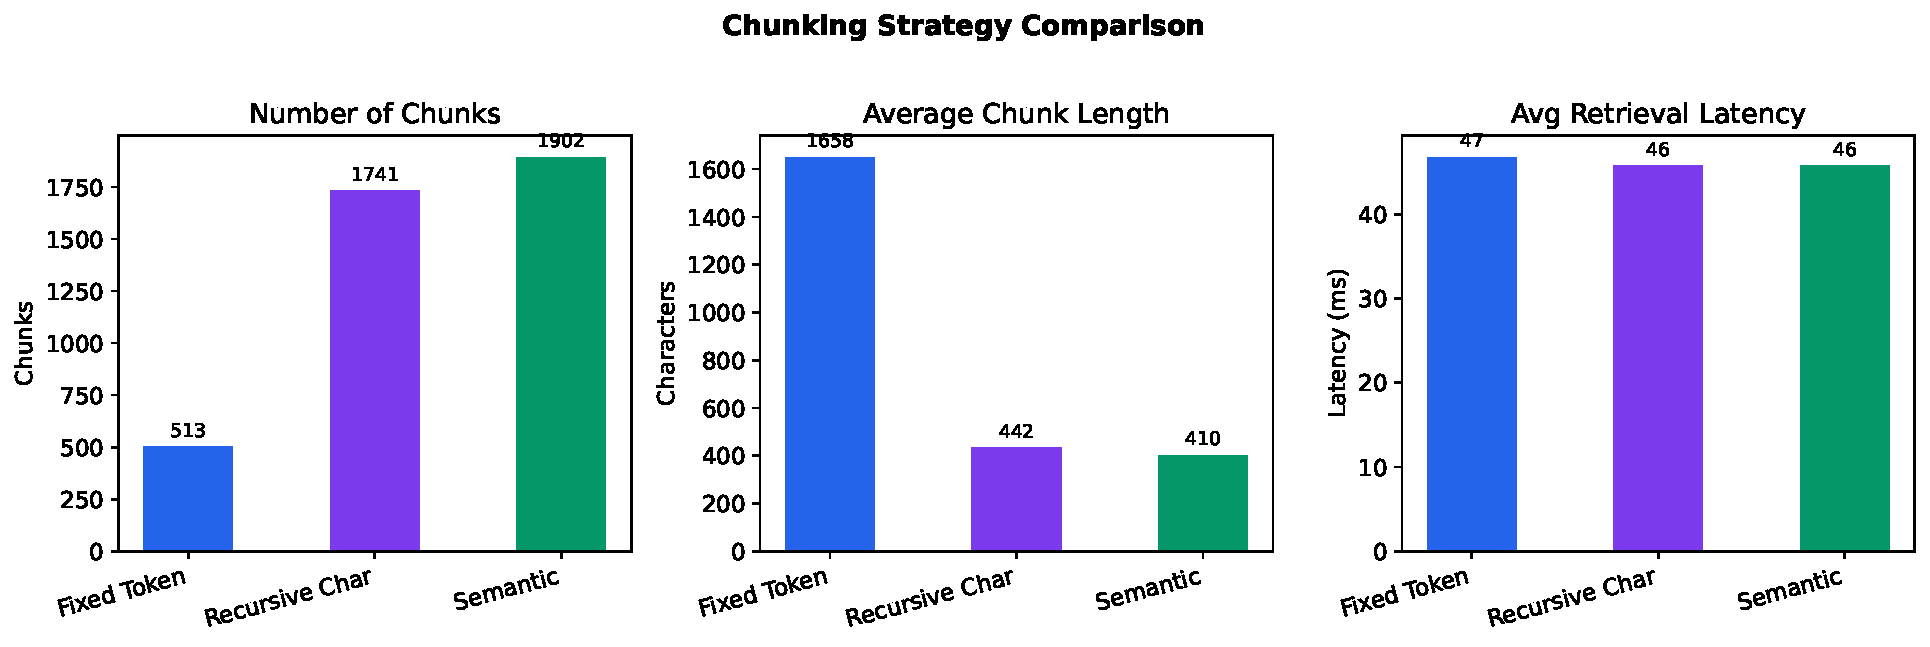
\includegraphics[width=\textwidth]{figures/chunking_comparison.pdf}
\caption{分块策略对比——三种策略在分块数、平均长度和检索延迟三个维度上的差异。Fixed Token（固定Token分块）产生较少较大块，Semantic（语义分块）产生较多较小块。}
\label{fig:chunking}
\end{figure}

\begin{figure}[htbp]
\centering
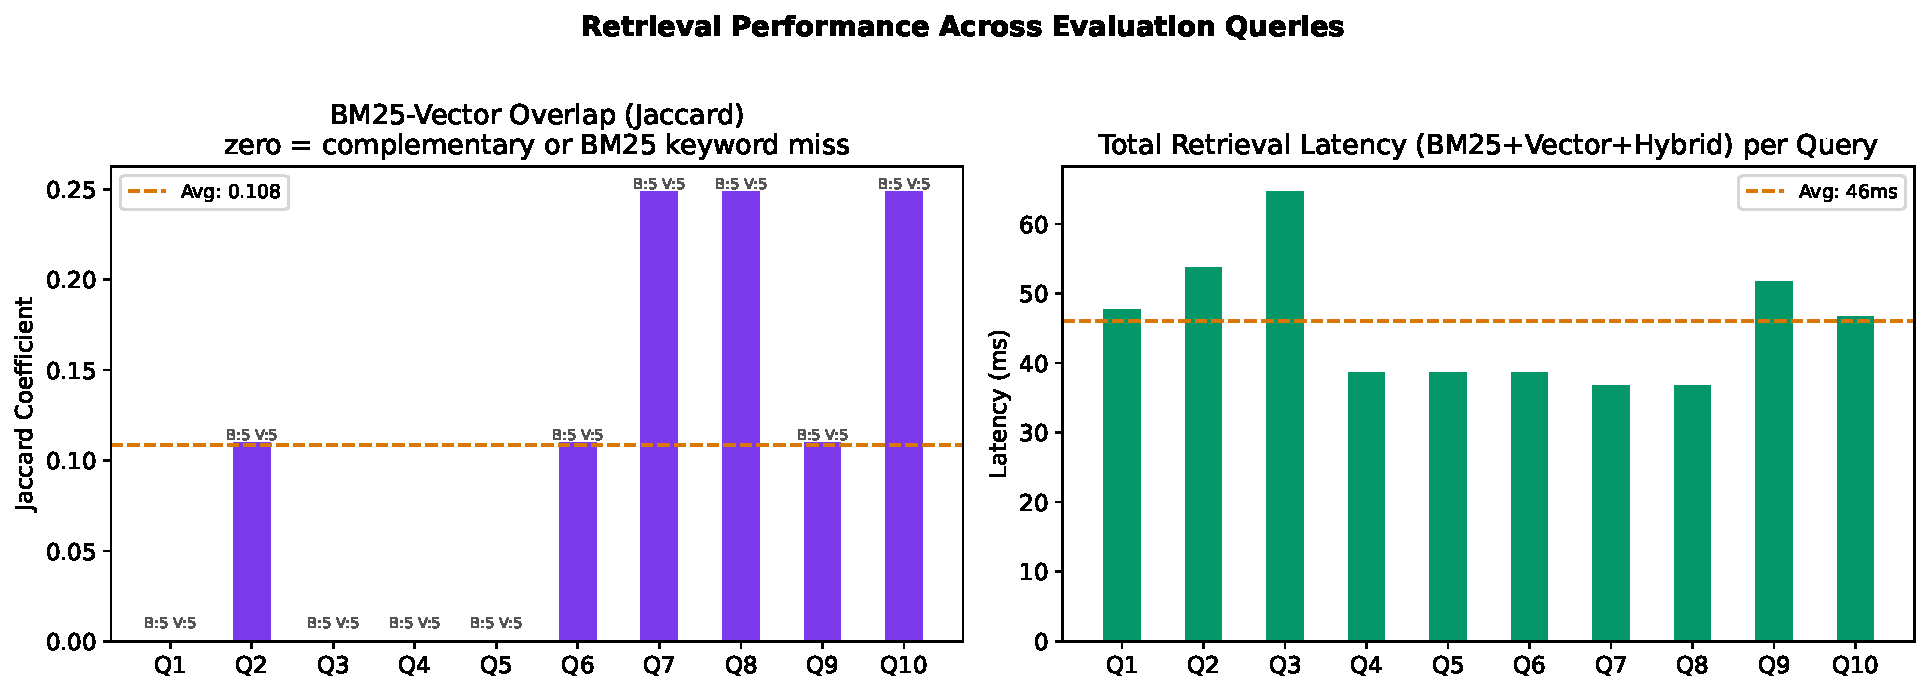
\includegraphics[width=\textwidth]{figures/retrieval_performance.pdf}
\caption{检索性能逐查询分析——BM25与向量检索的Jaccard重叠度（左，bar上标注BM25/向量检索结果数，零值=BM25关键词未命中或两者不重叠）和检索延迟（右）。低重叠度表明两种检索方式各有所长、互为补充。}
\label{fig:retrieval}
\end{figure}

\begin{figure}[htbp]
\centering
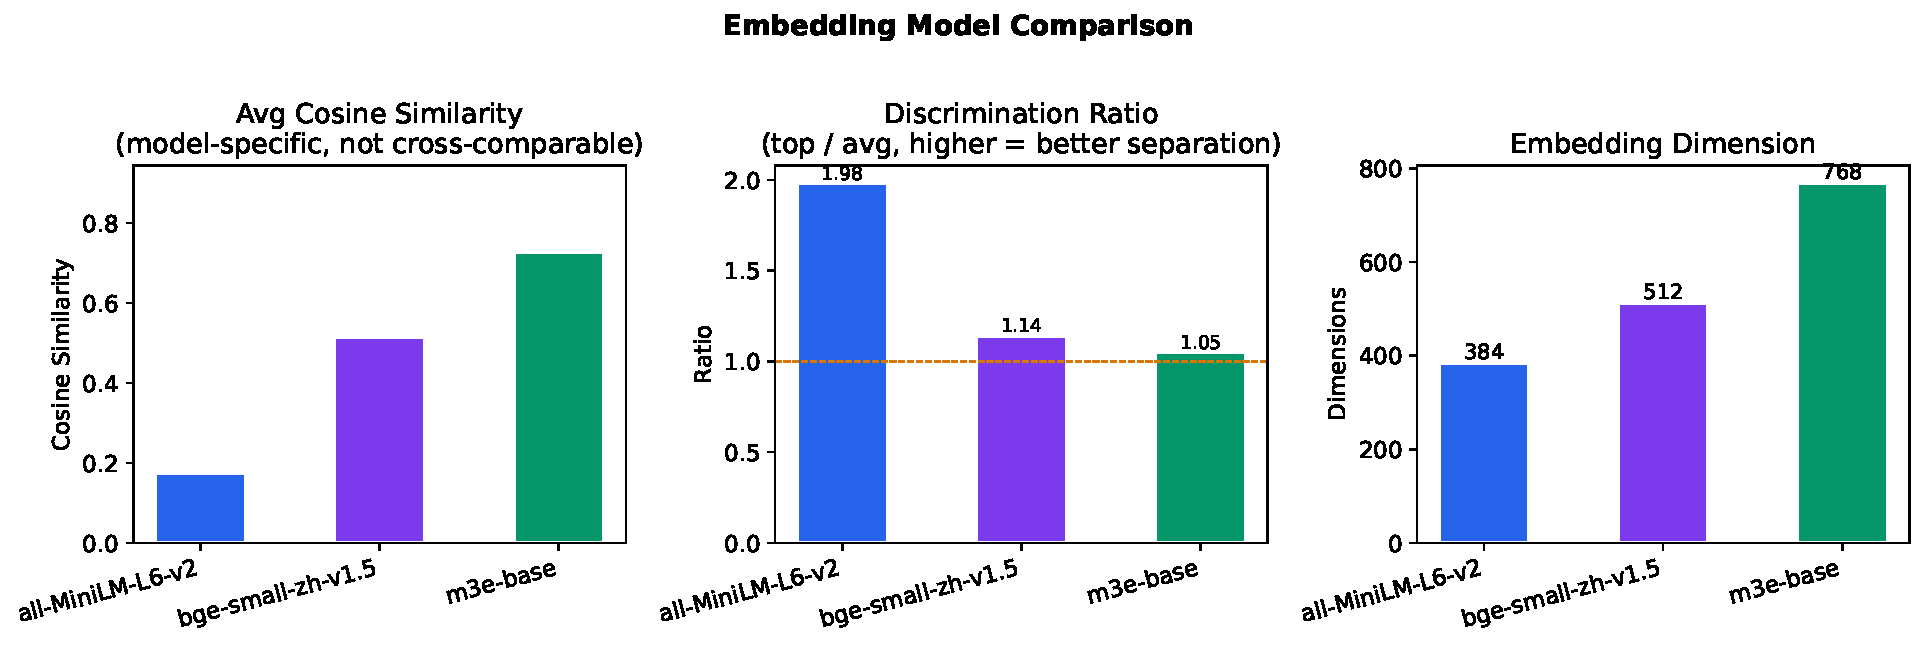
\includegraphics[width=\textwidth]{figures/embedding_comparison.pdf}
\caption{嵌入模型对比——三种模型在余弦相似度均值（模型特异性指标，不可跨模型直接比较）、区分度比率（最佳匹配/平均相似度，$>$1表示有效区分，可跨模型比较）和向量维度上的表现。MiniLM（384维）作为轻量模型保持了良好的区分能力，M3E（768维）以更高维度提供更大的语义容量。}
\label{fig:embedding}
\end{figure}

\begin{figure}[htbp]
\centering
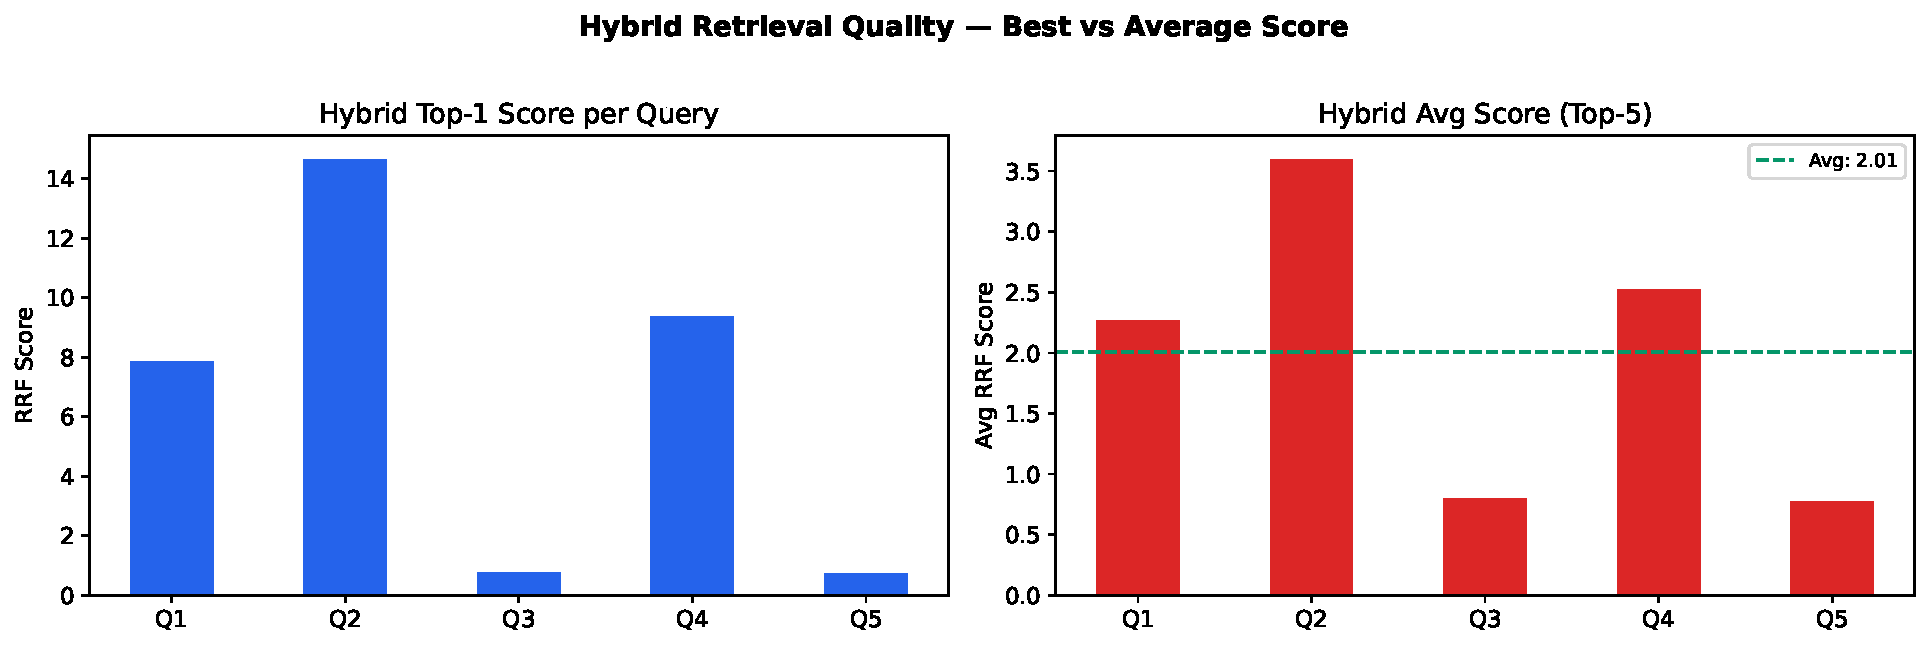
\includegraphics[width=\textwidth]{figures/hybrid_quality.pdf}
\caption{混合检索质量——Top-1融合得分（左）和Top-5平均融合得分（右）。两图共同展示了每次查询中最佳结果与整体结果集的质量差异。在RRF模式下为RRF融合分，在加权模式下为加权融合分。}
\label{fig:hybrid_quality}
\end{figure}

\begin{figure}[htbp]
\centering
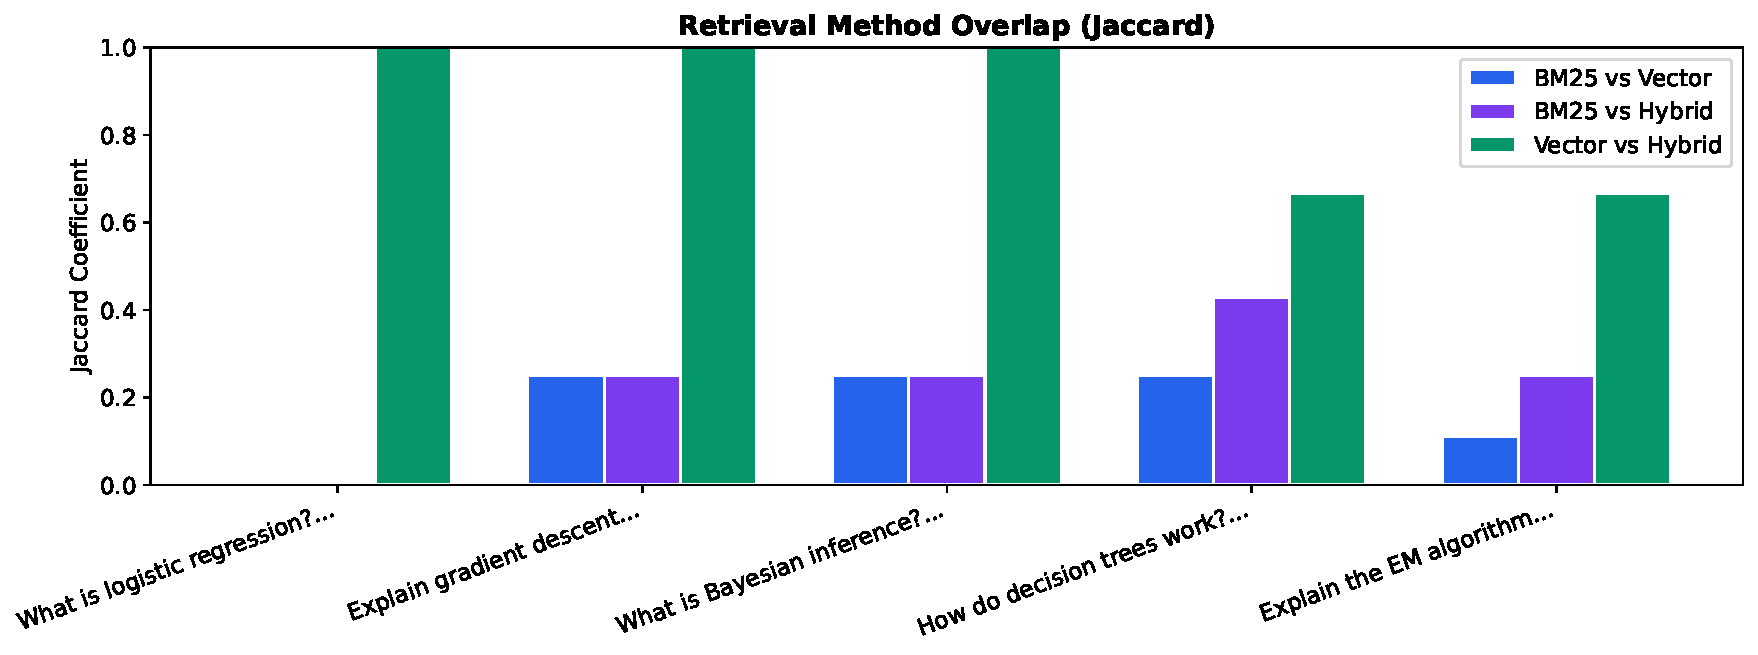
\includegraphics[width=\textwidth]{figures/retrieval_methods.pdf}
\caption{检索方式重叠度——BM25、向量、混合三种检索方式两两之间的Jaccard重叠度。BM25与向量检索重叠度最低，说明两者抓取了不同的相关文档，这正是混合检索互补设计的依据。}
\label{fig:retrieval_methods}
\end{figure}

\subsubsection{评估查询列表}

系统使用以下10条机器学习核心概念查询进行标准化评估（在config.py中通过eval\_queries配置，可替换为自定义查询）：

\begin{table}[htbp]
\centering
\begin{tabular}{@{}cl@{}}
\toprule
\textbf{编号} & \textbf{评估查询} \\
\midrule
Q1  & What is logistic regression? \\
Q2  & Explain the concept of support vector machines \\
Q3  & What is the bias-variance tradeoff? \\
Q4  & How does gradient descent work? \\
Q5  & What is cross-validation? \\
Q6  & Explain the EM algorithm \\
Q7  & What is Bayesian inference? \\
Q8  & How do decision trees work? \\
Q9  & What is the difference between supervised and unsupervised learning? \\
Q10 & Explain principal component analysis \\
\bottomrule
\end{tabular}
\caption{标准化评估查询列表——覆盖机器学习核心概念，用于系统各项评估指标的计算与对比}
\label{tab:eval_queries}
\end{table}

\subsubsection{自动化测试套件}

为保障系统代码质量与后续维护的可靠性，本项目建立了基于 pytest 框架的自动化单元测试与集成测试套件，共计 81 个测试用例（77 通过，4 跳过），覆盖以下六大核心模块：

\begin{enumerate}[label=(\arabic*)]
\item \textbf{文本分块模块（test\_chunker.py，17 个用例）：}测试三种分块策略（FixedTokenChunker、RecursiveCharChunker、SemanticChunker）的切分正确性、边界条件（空文本、短文本）、分块大小约束、元数据完整性、策略切换、策略对比统计功能。
\item \textbf{向量嵌入模块（test\_embedder.py，6 个用例）：}验证嵌入向量维度与模型一致、批量嵌入与单条嵌入的数组形状、L2 归一化正确性（范数值约 1.0）、相同文本产生相同嵌入的一致性、相关文本与不相关文本的相对区分度。
\item \textbf{混合检索模块（test\_retriever.py，22 个用例）：}覆盖中英文检测与分词、RRF 排名融合算法数学正确性（含排名合并、权重计算、Top-K 截断）、加权融合归一化逻辑、BM25 关键词检索集成、向量语义检索集成、混合检索集成、查询翻译缓存机制。
\item \textbf{向量存储模块（test\_vector\_store.py，9 个用例）：}验证 ChromaDB 的增删查功能、向量计数、清除与重建（防止数据污染）、FAISS 存储（可选，依赖 FAISS 安装）、异常存储类型报错。
\item \textbf{系统评估模块（test\_evaluator.py，13 个用例）：}验证检索评估结果数据结构与字段完整性、RRF融合得分正确选择、空检索边界处理、分块策略对比后的Pipeline状态恢复、生成质量评估中LLM实际调用（use\_llm=True）、完整评估流程四阶段执行、格式化报告输出。
\item \textbf{LLM生成模块（test\_generator.py，14 个用例）：}验证三种LLM提供商初始化、上下文文档格式化、降级回复模板、提示词模板渲染、生成结果数据结构完整性、API调用中上下文正确传入、API异常向上传播、本地模型路由。
\end{enumerate}

测试运行命令：

\begin{verbatim}
pytest tests/ -v                        # 运行全部测试
pytest tests/ -v -k "not Integration"   # 仅快速单元测试
pytest tests/ --cov=src --cov-report=term-missing  # 查看覆盖率
\end{verbatim}

测试套件运行结果：77 个用例通过，4 个跳过（FAISS 未安装），0 个失败，执行耗时约 34 秒（含嵌入模型加载）。新增的评估与生成模块测试使用 mock 隔离外部依赖，在不调用真实 LLM API 的前提下完整验证核心逻辑。测试采用离线模式加载嵌入模型（HF\_HUB\_OFFLINE=1），从本地缓存即时加载，避免网络延迟。

% ============================================================
% 第5章 总结
% ============================================================
\section{总结}

\subsection{任务执行情况}

本项目按照前期制定的开发计划，顺利完成了RAG-Lab检索增强生成实验系统的全部设计与实现工作。各项任务完成情况如下：

\begin{enumerate}[label=(\arabic*)]
\item 文档获取与解析模块：实现了CMU课程网页自动抓取、PDF批量下载与解析、文本清洗与JSON缓存功能，内置10篇示例文档确保离线可用
\item 文本分块模块：实现了固定Token分块、递归字符分块、语义分块三种策略，支持chunk\_size和chunk\_overlap灵活配置
\item 向量嵌入模块：集成了MiniLM、BGE、M3E三种Sentence-Transformers嵌入模型，支持批量嵌入与单条查询嵌入，提供模型对比工具函数
\item 向量存储模块：实现了ChromaDB持久化存储和FAISS内存存储两种后端，统一add/query接口，支持清除重建
\item 混合检索模块：实现了BM25关键词检索（含中文分词与跨语言翻译）与向量语义检索的混合方案，支持RRF排名融合和加权求和两种融合策略，并提供三种检索方式的独立对比功能
\item LLM生成模块：实现了基于检索文档的答案生成，支持DeepSeek和OpenAI两种API后端，采用结构化提示词模板与降级容错机制
\item 评估模块：实现了检索质量、分块策略、嵌入模型、生成质量四维度评估，内置10条机器学习核心概念评估查询
\item 交互界面：实现了CLI命令行界面（5个子命令）和Gradio网页界面（4个功能页签），兼顾开发效率与演示效果
\end{enumerate}

全部核心功能模块均按时并高质量完成，各项功能运行正常，达到了预期的设计目标。

\subsection{工作态度与质量表现}

在本项目的开发过程中，展现了良好的工作态度和高度的责任心。从项目选题、需求分析、系统设计到代码实现和测试验证的每个阶段，认真查阅相关资料和文档。在技术选型方面，经过充分比较选择了最适合RAG学习场景的开源技术栈（ChromaDB的易用性、Gradio的可交互性、BGE的中文嵌入能力等）。在代码编写方面，注重模块化设计和可读性，全局配置集中管理，关键参数附带详细注释说明，保证了代码的规范性和可维护性。

\subsection{团队协作与沟通}

本项目为个人独立完成。在开发过程中，充分利用了开源社区资源（GitHub、模型文档、API文档），通过阅读官方文档与技术博客解决了嵌入模型加载、ChromaDB持久化配置、Gradio自定义CSS等技术难题。同时，项目预留了丰富的扩展接口，便于后续团队协作——其他开发者可在此基础上进行功能扩展。

\subsection{贡献表}

本项目各模块均由个人独立完成，具体贡献如下：

\vspace{6pt}

\begin{longtable}{@{}|p{3.5cm}|p{12cm}|@{}}
\toprule
\textbf{模块} & \textbf{贡献描述} \\
\midrule
\endfirsthead
\toprule
\textbf{模块} & \textbf{贡献描述} \\
\midrule
\endhead
\bottomrule
\endfoot
\bottomrule
\endlastfoot
项目架构设计 & 设计了RAG流水线六阶段模块化架构，制定了各模块的接口规范与协作关系 \\
config.py & 设计了基于dataclass的集中化配置管理方案，涵盖路径、分块、嵌入、存储、检索、生成、评估七大配置域，支持环境变量注入 \\
document\_loader.py & 实现了CMU课程网页抓取、PDF/HTML解析、JSON缓存、内置示例文档生成等完整功能 \\
chunker.py & 实现了策略模式的三种分块策略（FixedTokenChunker / RecursiveCharChunker / SemanticChunker）及策略对比功能 \\
embedder.py & 封装了sentence-transformers模型加载、批量嵌入、查询嵌入及多模型对比工具 \\
vector\_store.py & 实现了ChromaDB和FAISS双后端的统一向量存储接口 \\
retriever.py & 实现了BM25关键词检索（含中文分词、查询翻译）、向量检索、RRF/加权双模式融合及检索方式对比功能 \\
generator.py & 实现了LLM答案生成（DeepSeek/OpenAI API）、结构化提示词模板、降级容错机制 \\
evaluator.py & 实现了检索质量、分块策略、嵌入模型、生成质量四维度评估及格式化报告输出功能 \\
app.py & 基于Gradio构建了包含智能问答、检索对比、系统评估、关于系统四个页签的Web界面，自定义CSS样式 \\
main.py & 基于argparse实现了CLI命令行界面及5个子命令 \\
tests/ & 建立了包含81个用例的pytest自动化测试套件，覆盖六大核心模块（分块、嵌入、检索、存储、评估、生成），包含mock隔离与集成测试 \\
README.md & 编写了完整的项目说明文档，包括项目背景、快速开始、CLI命令一览、教程路线、技术栈、配置说明等 \\
\end{longtable}

项目总代码量约2800行（Python），包含10个功能源文件和7个测试文件，共81条测试用例。

\subsection{总结}

通过本次RAG-Lab项目的开发与实践，深入掌握了检索增强生成（RAG）技术的核心原理与工程实现方法。项目从底层实现了RAG流水线的每个环节，对文档处理、文本分块策略、向量嵌入模型、向量数据库、混合检索融合、提示词工程等关键技术有了深入而具体的理解。

在技术层面，实践掌握了多项技能：使用sentence-transformers进行文本向量化处理，使用ChromaDB和FAISS构建高效的向量检索系统，使用BM25与向量混合策略提升检索质量，使用Gradio构建交互式机器学习应用界面，使用argparse开发用户友好的命令行工具。

在工程层面，本项目践行了模块化设计、策略模式、配置集中化管理、容错降级等软件工程实践，使代码结构清晰、可维护性强、便于扩展。项目内置的评估体系使得不同策略和模型的性能差异可以通过量化指标进行客观比较，培养了数据驱动的系统优化思维。

本项目的优化方向：（1）实现Re-Ranker重排序，检索精度可进一步提升；（2）支持多轮对话记忆；这些将作为后续版本迭代的改进方向。流式输出（Streaming）已在 v1.1 版本中实现，可在 Gradio 网页界面中实时逐字展示 LLM 回答。

总体而言，本次实践达到了预期的学习目标，成功构建了一个功能完整、交互友好、教学价值突出的RAG实验系统，为今后构建更复杂的RAG应用奠定了坚实的理论与实践基础。

项目全部源码、部署教程与实验文档均已开源，可访问对应仓库查看完整项目\footnote{项目开源地址：\url{https://github.com/jmdonbaba/RAG-Lab}}。



\begin{flushright}
\vspace{2\baselineskip}

{\large 2026年5月11日}

\end{flushright}
\end{document}
